\documentclass[a4paper, 12pt]{article}
\usepackage[top=2cm, bottom=2cm, left=2.5cm, right=2.5cm]{geometry}
\usepackage[utf8]{inputenc}
\usepackage[brazilian]{babel}
\usepackage{indentfirst}
\usepackage{graphicx}
\usepackage{wrapfig}
\usepackage[pdftex]{hyperref}
\usepackage{amsmath}
\usepackage{subcaption}

\begin{document}
	\begin{center} %centralizar o texto abaixo
		{\Large Exponencial matricial e simulação com representação de estados}\\[0.4cm]
		{\large Erik Yuji Goto}\\[0.2cm]
		{\normalsize RA: 234009}
	\end{center} %término do comando centralizar

\section{Sistema de Segunda Ordem}
	A equação do movimento escrita na forma padronizada é:	
	\begin{equation}
		\ddot{q} + 2\xi \omega_n \dot{q} + \omega_n^2q = \omega_n^2u(t)
	\end{equation}
	Substituindo pelos valores do enunciado:	
	\begin{equation}
		\ddot{q} + 10\dot{q} + 10^4q = 0
	\end{equation}
	Com isso podemos transformar a equação para a forma matricial:
	\begin{figure}[h]
		\centering
		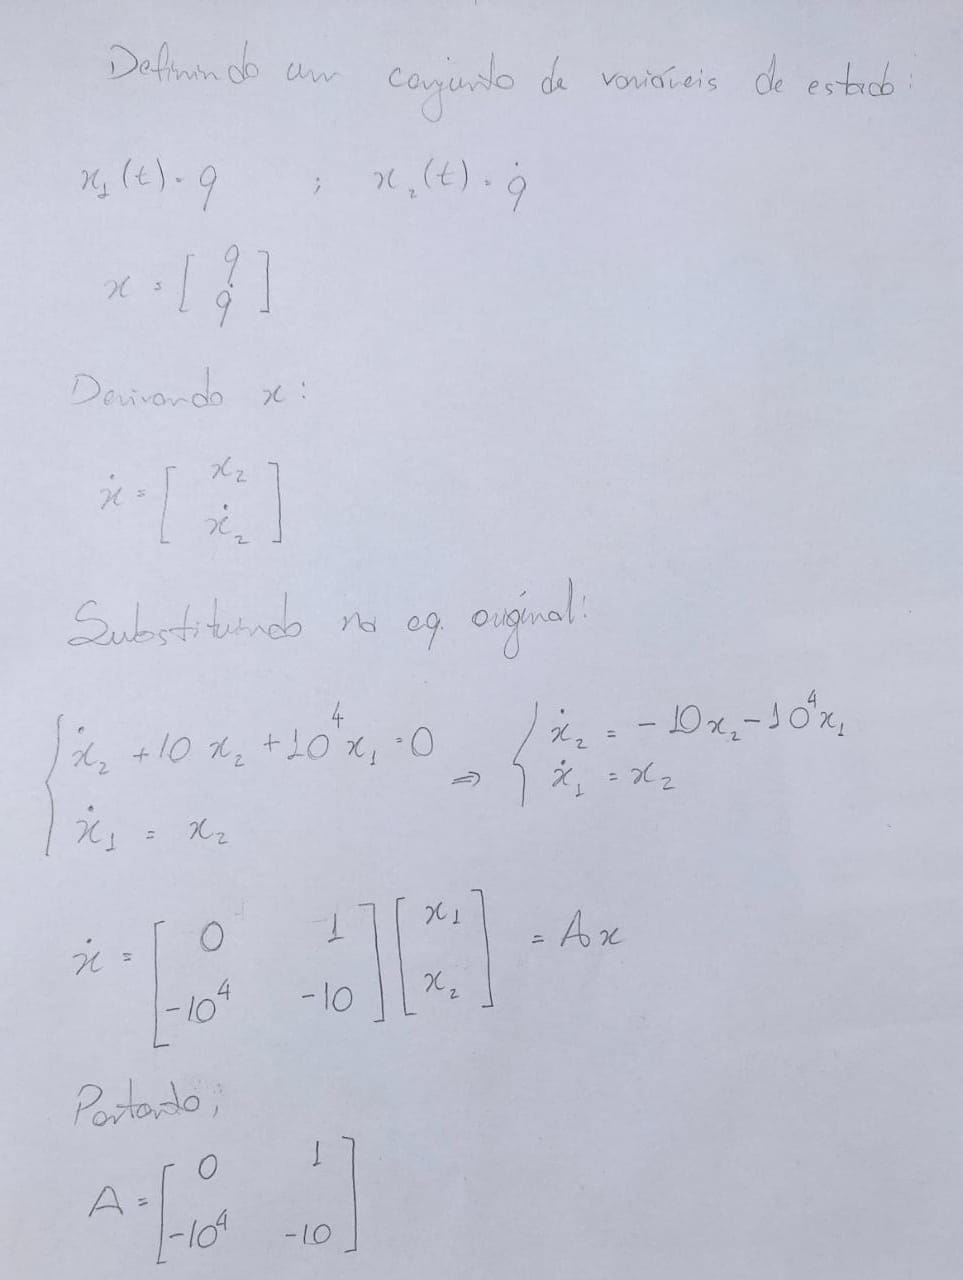
\includegraphics[scale=0.35]{imagens/a1.jpg}
		\caption{Encontrando a matriz A}
	\end{figure}
	\newpage
	Portanto,
	\begin{equation}
		\dot{x} = Ax + Bu
	\end{equation}
	Onde,
	\begin{equation}
		Bu = 0
	\end{equation}
	\begin{equation}
		A = \begin{bmatrix}
		0 & 1\\
		-10^4 & -10
		\end{bmatrix}
	\end{equation}

\section{Calculando a resposta livre}
	A resposta livre a uma condição inicial é dada por:
	\begin{equation}
		x(t) = e^{At} x_0
	\end{equation}
	Portanto, precisamos calcular $e^{At}$
	
	\subsection{Por Autovalores}
		\begin{figure}[h]
			\centering
			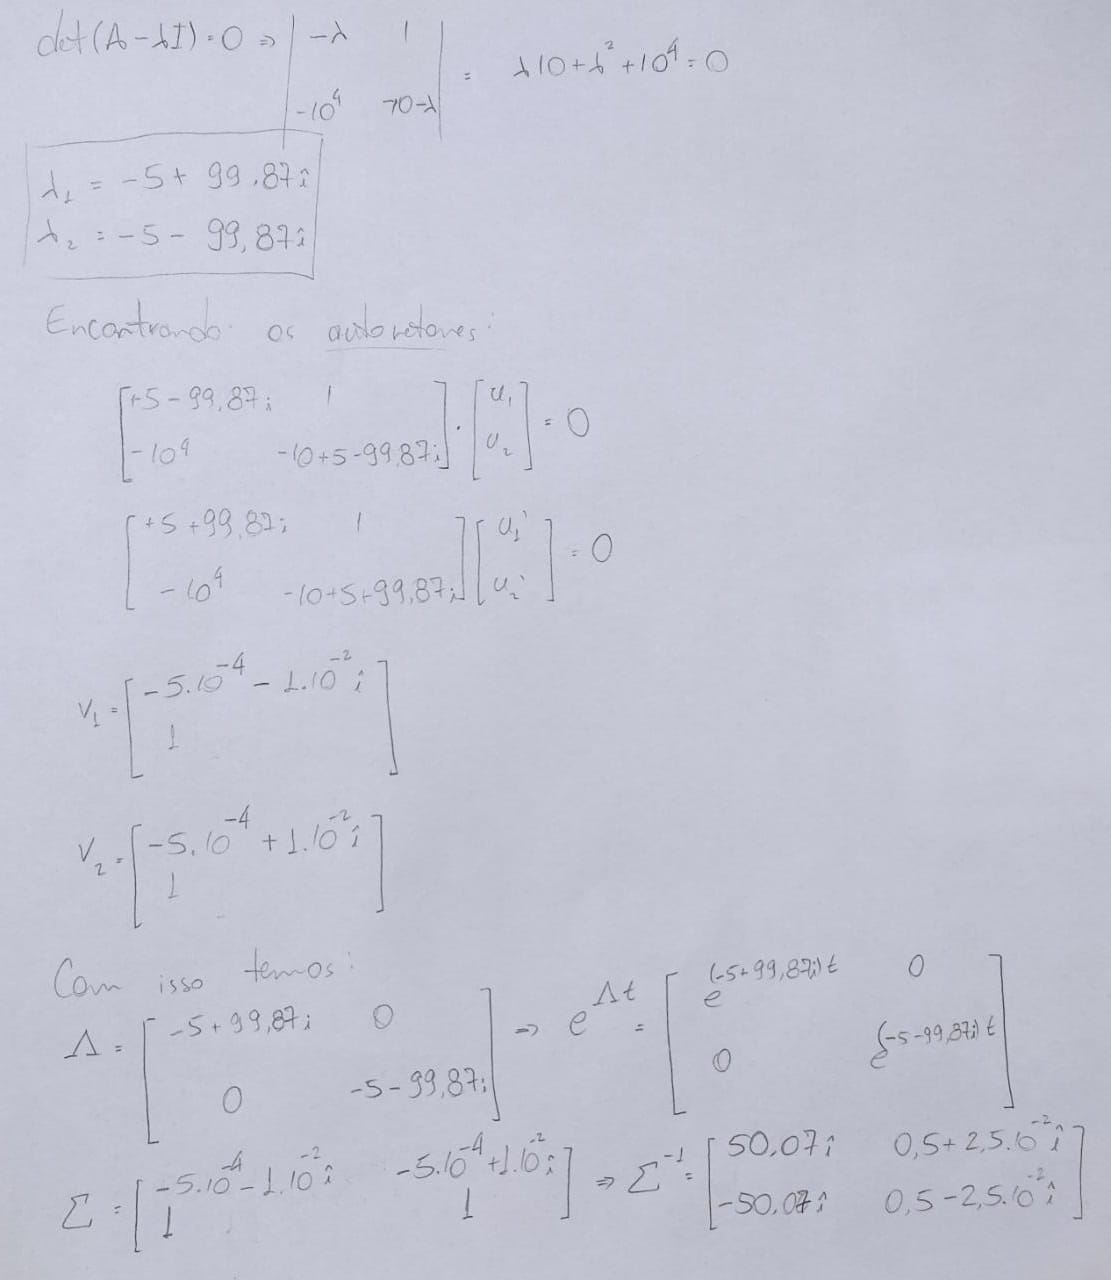
\includegraphics[scale=0.3]{imagens/a2.jpg}
			\caption{Autovalores}
		\end{figure}
		Realizando o cálculo de $e^{At}$ pelo matlab:
		\begin{center}
			$syms \texttt{ t};$\\
			$[U,L] = eig(A);$\\
			$e^{At} = U*diag(exp(diag(L*t)))*inv(U)$\\
		\end{center}				
		
		\begin{equation}
			e^{At} = \begin{bmatrix}
				a & b\\
				c & d
			\end{bmatrix}
		\end{equation}
		Onde,\\
		
		$a = exp(t*(- 5 + 399^{(1/2)}*5i))*(\frac{1}{2} - 0.0250i)+ exp(-t*(5 + 399^(1/2)*5i))*(\frac{1}{2} + 0.0250i)$\\
		
		$b = - exp(t*(- 5 + 399^(1/2)*5i))*(10001^{(1/2)}/200 + 0.0250i)*(5*10^{-4} + 0.01i) - exp(-t*(5 + 399^{(1/2)}*5i))*(10001^{(1/2)}/200 - 0.0250i)*(5*10^{-4} - 0.01i)$\\
		
		$c = 10001^{(1/2)}*exp(t*(- 5 + 399^{(1/2)}*5i))*0.5i - 10001^{(1/2)}*exp(-t*(5 + 399^(1/2)*5i))0.5i$\\
		
		$d = (100*10001^(1/2)*exp(t*(- 5 + 399^(1/2)*5i))*(10001^(1/2)/200 + 0.025i))/10001 + (100*10001^(1/2)*exp(-t*(5 + 399^(1/2)*5i))*(10001^(1/2)/200 - 0.025i))/10001$\\
		

	\subsection{Por Laplace}
		Usaremos a relação $e^{At} = L^{-1}[(sI-A)^{-1}]$
		\begin{figure}[h]
			\centering
			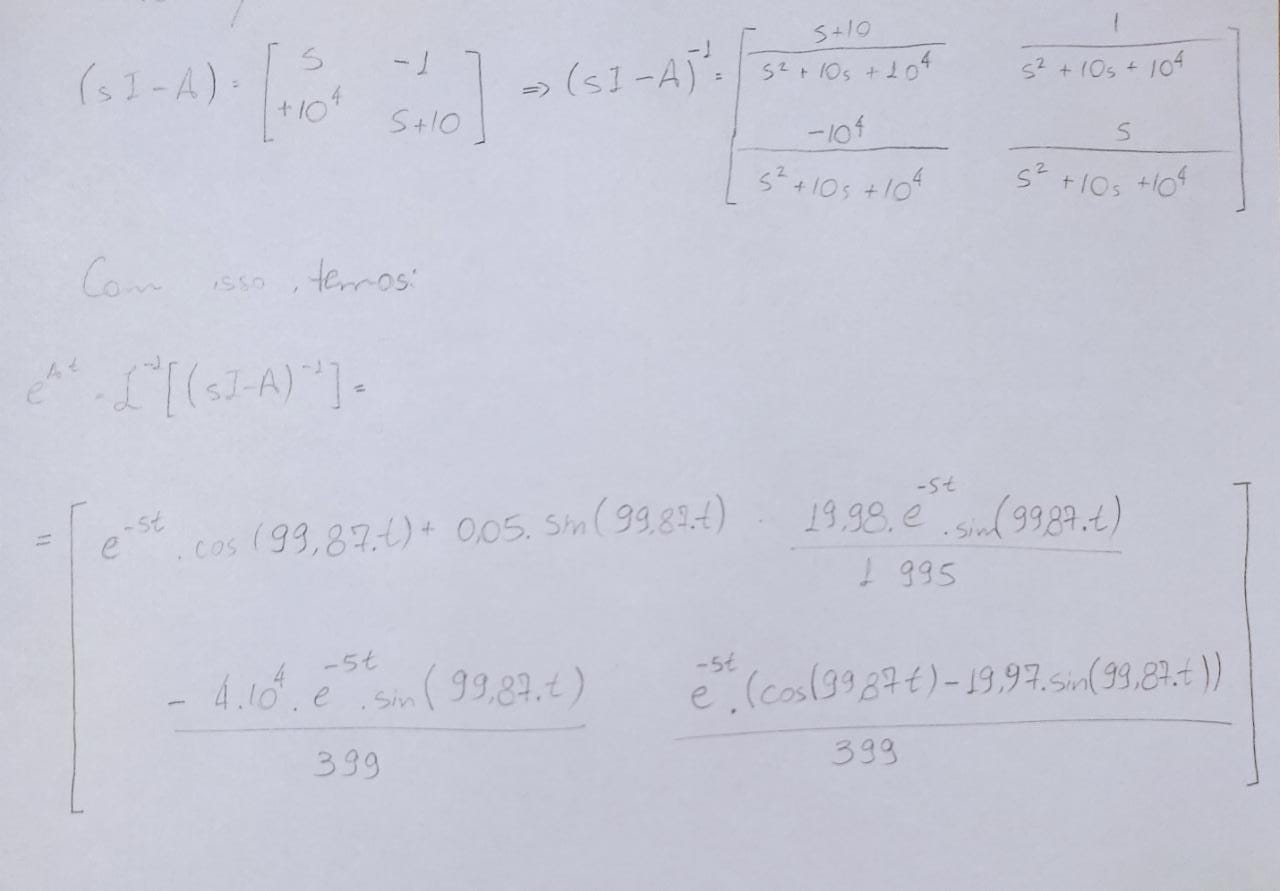
\includegraphics[scale=0.3]{imagens/a3.jpg}
			\caption{Laplace}
		\end{figure}
		
	\subsection{Por Cayley-Hamilton}
		Usamos a equação $e^{At} = \sum^{n-1}_{l = 0} \alpha_lA^l$
		Para encontrar as constantes $\alpha_l$ resolvemos o sistema de equações:
		\begin{figure}[h]
			\centering
			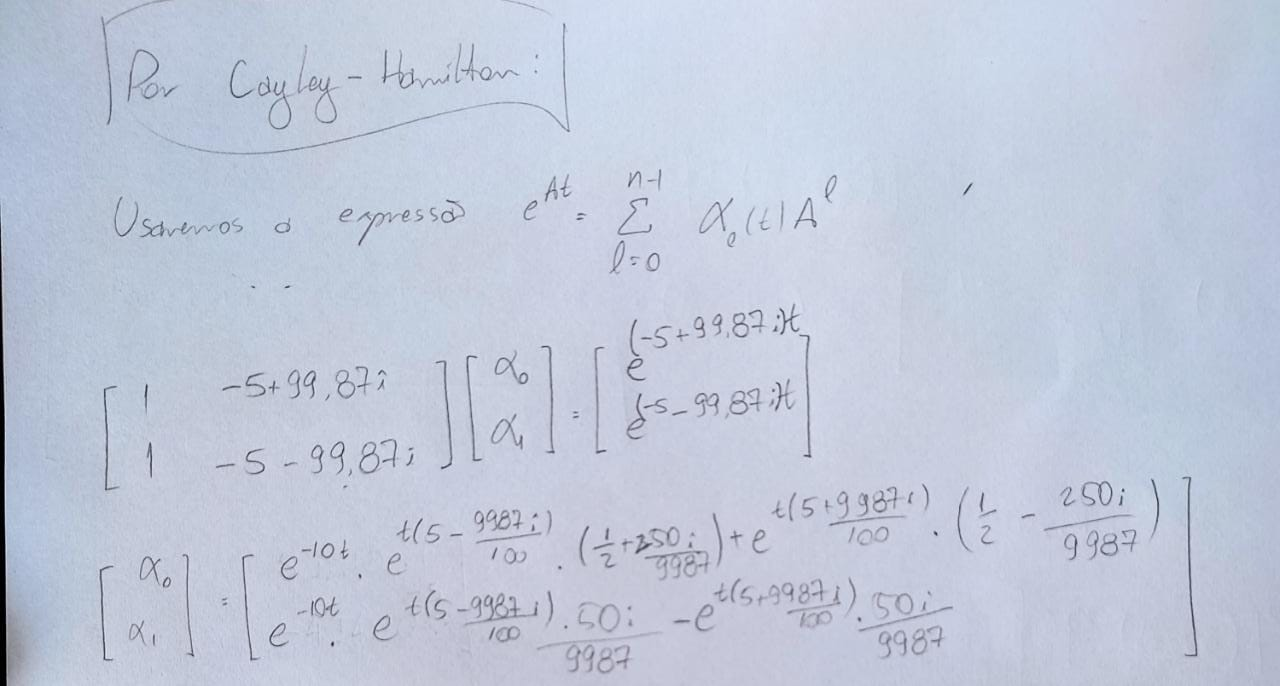
\includegraphics[scale=0.3]{imagens/a4.jpg}
			\caption{Cayley-Hamilton}
		\end{figure}\\
		Pelo Matlab, calculamos $e^{At} = \alpha_0I + \alpha_1A$:
		\begin{equation}
			e^{At} = \begin{bmatrix}
				a & b\\
				c & d
			\end{bmatrix}
		\end{equation}
		Onde,\\
		$a = exp(-10*t)*(exp(t*(5 - 9987i/100))*(1/2 + 250i/9987) + exp(t*(5 + 9987i/100))*(1/2 - 250i/9987))$\\
		
		$b = exp(-10*t)*((exp(t*(5 - 9987i/100))*50i)/9987 - (exp(t*(5 + 9987i/100))*50i)/9987)$\\
		
		$c = -10000*exp(-10*t)*((exp(t*(5 - 9987i/100))*50i)/9987 - (exp(t*(5 + 9987i/100))*50i)/9987)$\\
		
		$d = exp(t*(- 5 - 9987i/100))*(1/2 - 250i/9987) + exp(t*(- 5 + 9987i/100))*(1/2 + 250i/9987)$

	\subsection{Por expm}
		Pelo comando \textit{expm(A*t)} é possível calcular a exponencial matricial, portanto a resposta livre:
		\begin{equation}
			e^{At} = \begin{bmatrix}
				a & b\\
				c & d
			\end{bmatrix}
		\end{equation}
		Onde,\\
		$a = exp(- 5*t - 399^{(1/2)}*t*5i)/2 + exp(- 5*t + 399^{(1/2)}*t*5i)/2 + (399^{(1/2)}*exp(- 5*t - 399^{(1/2)}*t*5i)*1i)/798 - (399^{(1/2)}*exp(- 5*t + 399^{(1/2)}*t*5i)*1i)/798$\\
		
		$b = (399^{(1/2)}*exp(- 5*t - 399^{(1/2)}*t*5i)*1i)/3990 - (399^{(1/2)}*exp(- 5*t + 399^{(1/2)}*t*5i)*1i)/3990$\\
		
		$c = -(399^{(1/2)}*exp(- 5*t - 399^{(1/2})*t*5i)*1000i)/399 + (399^{(1/2)}*exp(- 5*t + 399^{(1/2)}*t*5i)*1000i)/399$	\\
		
		$d = exp(- 5*t - 399^{(1/2)}*t*5i)/2 + exp(- 5*t + 399^{(1/2)}*t*5i)/2 - (399^{(1/2)}*exp(- 5*t - 399^{(1/2)}*t*5i)*1i)/798 + (399^{(1/2)}*exp(- 5*t + 399^{(1/2)}*t*5i)*1i)/798$

\newpage
\section{Simulink e Resposta forçada}
	Primeiro vamos definir as matrizes A, B, C e D. \\
	A foi definido anteriormente.
	Já a matriz B usaremos o fato de que:
	\begin{equation}
		\ddot{q}= \omega_n^2u(t) - 2\xi \omega_n \dot{q} - \omega_n^2q 
	\end{equation}
	\begin{equation}
		\dot{x} = Ax + Bu
	\end{equation}
	Portanto, 
	\begin{equation}
		B = \begin{bmatrix}
			0\\
			\omega_n^2			
		\end{bmatrix} = \begin{bmatrix}
			0\\
			10^4
		\end{bmatrix}
	\end{equation}
	Suponha que a resposta desejada seja a posição e a velocidade, então as matrizes C e D ficam sendo:
	\begin{equation}
		C = \begin{bmatrix}
			1\\
			1
		\end{bmatrix}
	\end{equation}
	\begin{equation}
		D = \begin{bmatrix}
			0\\
			0 
		\end{bmatrix}
	\end{equation}

	Para uma entrada degrau $u(t) = \mu(t)$, e condições iniciais $x_0 = \begin{bmatrix}
	1 \\ 5
	\end{bmatrix}$ temos o seguinte diagrama de blocos no simulink: 
	\begin{figure}[h]
		\centering
		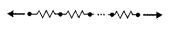
\includegraphics[scale=0.5]{imagens/a5.png}
		\caption{Simulink}
	\end{figure}\\
	\begin{figure}[h]
		\centering
		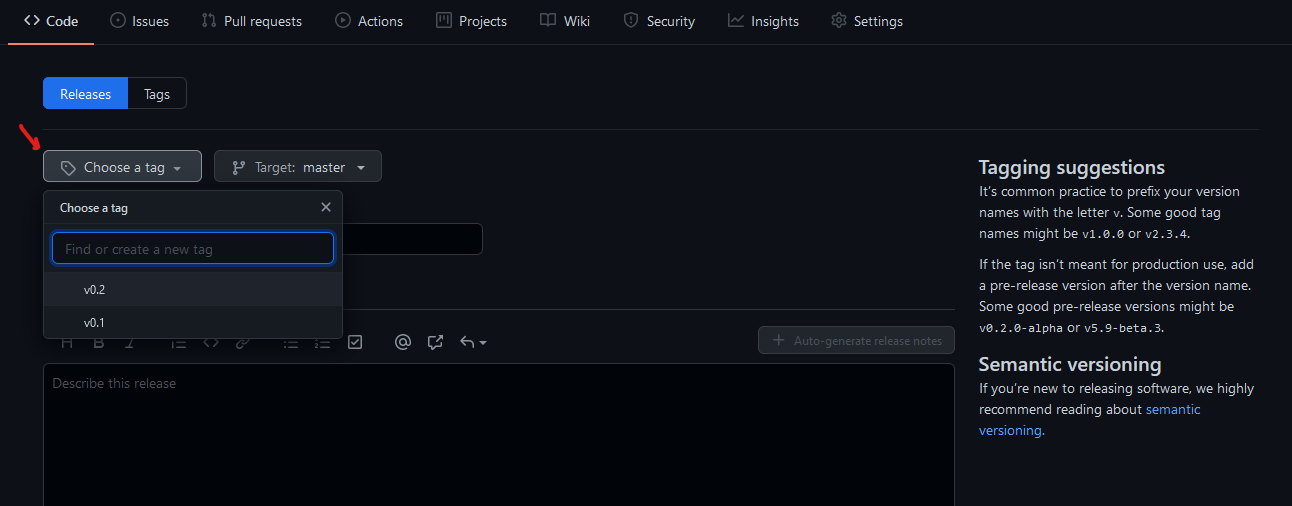
\includegraphics[scale=0.5]{imagens/a6.png}
		\caption{Configurações State-Space}
	\end{figure}\\
	\newpage
	Com a seguinte resposta:
	\begin{figure}[h]
		\centering
		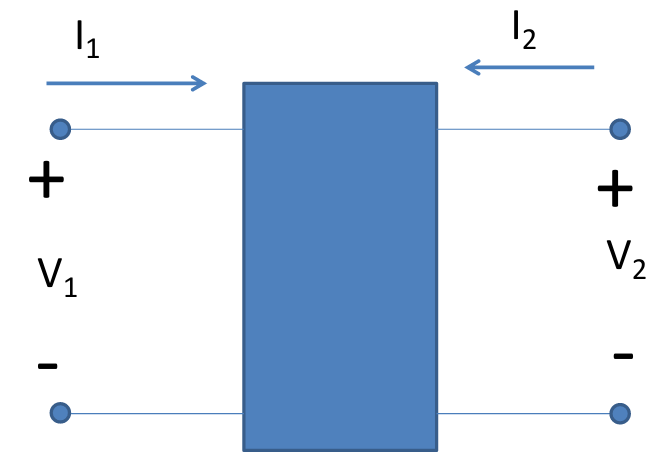
\includegraphics[scale=0.7]{imagens/a7.png}
		\caption{Resposta ao degrau}
	\end{figure}\\
	
\section{Funções ss, ss2tf e tf2ss}
	Pelo comando ss2tf conseguimos encontrar o denominador e o numerador da função transferência, usando como parâmetros as matrizes A, B, C e D:
	\begin{figure}[h]
		\centering
		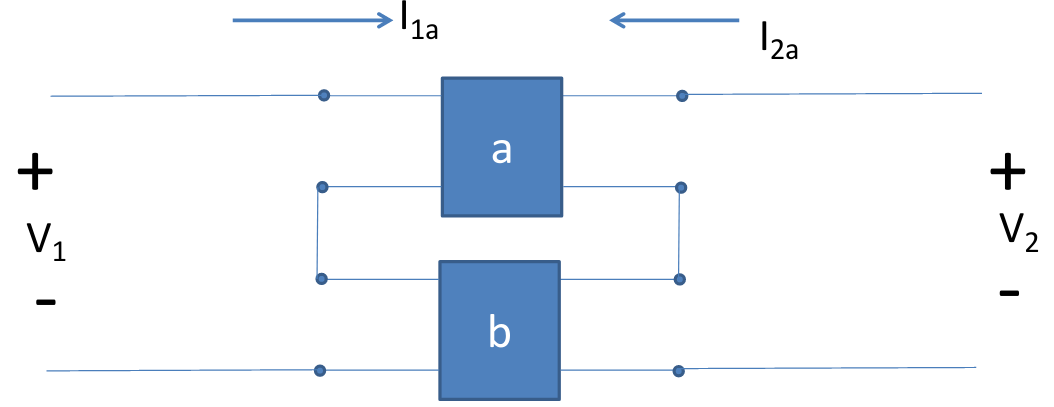
\includegraphics[scale=0.8]{imagens/a11.png}
		\caption{Função ss2tf}
	\end{figure}\\
	Disso, temos que a função transferência é:
		\begin{equation}
			H = \frac{1000s + 10^4}{s^2 + 10s + 10^4}
		\end{equation}
	\\
	
	Note que, pela propriedade da função transferência H não ser possível definir \textit{valores iniciais 	}, não conseguimos montar um diagrama de blocos para comparar os resultados usando o bloco \textit{Função transferência} e o bloco \textit{State-Space}, pois neste último definimos os valores iniciais $x_0 = \begin{bmatrix}
	1\\5	
	\end{bmatrix}
$.
	
	Caso já tivermos o valor da função transferência, e queremos resolver usando as matrizes de estado usamos o comando tf2ss:
	\begin{figure}[h]
		\centering
		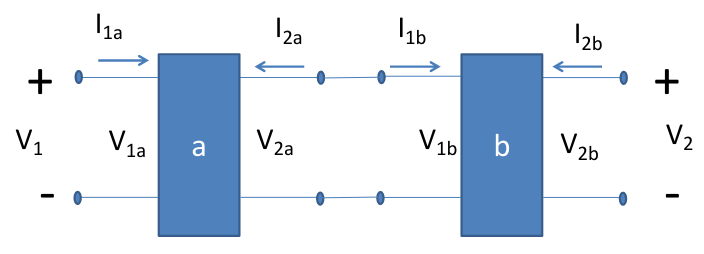
\includegraphics[scale=0.8]{imagens/a12.png}
		\caption{Função tf2ss}
	\end{figure}
	
	Ao executar esta linha, o resultado são as matrizes de estado:
	\begin{figure}[h]
		\centering
		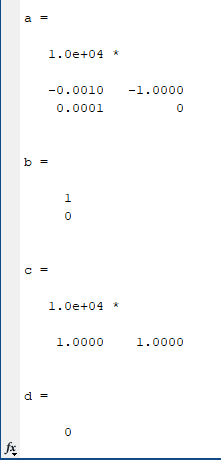
\includegraphics[scale=0.8]{imagens/a13.png}
		\caption{Matrizes de Estado}
	\end{figure}
	
	
	
	
\newpage	
\section{Usando o comando lsim}
	Uma maneira mais simples de encontrar a resposta do sistema sabendo as matrizes é pelo comando lsim:
	\begin{figure}[h]
		\centering
		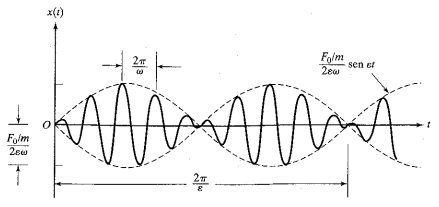
\includegraphics[scale=0.7]{imagens/a8.png}
		\caption{Solução usando lsim}
	\end{figure}\\
	\newpage
	E tem como resultado o seguinte plot
	\begin{figure}[h]
		\centering
		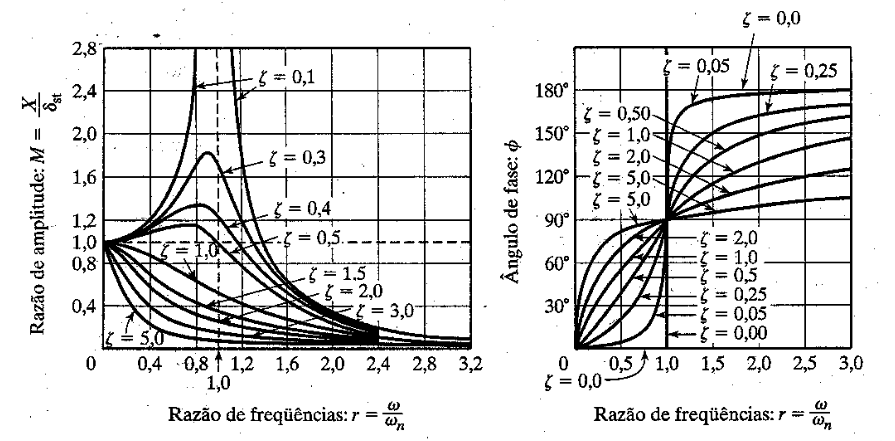
\includegraphics[scale=0.7]{imagens/a9.png}
		\caption{Plot usando lsim}
	\end{figure}
	\subsection{Comparação Simulink x lsim}
		Usando o simout conseguimos comparar o gráfico gerado pelo Simulink e pelo lsim
		\begin{figure}[h]
			\centering
			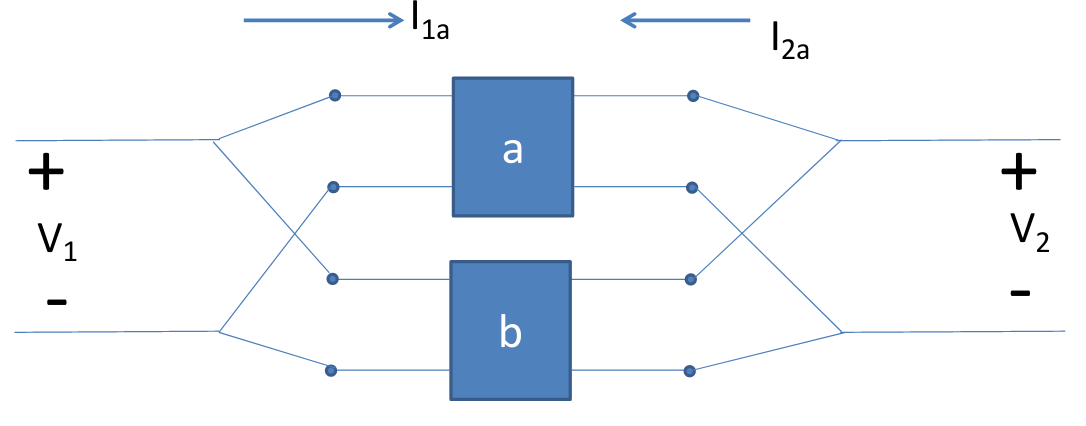
\includegraphics[scale=0.5]{imagens/a10.png}
			\caption{Plot comparação}
		\end{figure}
	
	
	
	
\end{document}